% Options for packages loaded elsewhere
\PassOptionsToPackage{unicode}{hyperref}
\PassOptionsToPackage{hyphens}{url}
%
\documentclass[
]{article}
\usepackage{lmodern}
\usepackage{amssymb,amsmath}
\usepackage{ifxetex,ifluatex}
\ifnum 0\ifxetex 1\fi\ifluatex 1\fi=0 % if pdftex
  \usepackage[T1]{fontenc}
  \usepackage[utf8]{inputenc}
  \usepackage{textcomp} % provide euro and other symbols
\else % if luatex or xetex
  \usepackage{unicode-math}
  \defaultfontfeatures{Scale=MatchLowercase}
  \defaultfontfeatures[\rmfamily]{Ligatures=TeX,Scale=1}
\fi
% Use upquote if available, for straight quotes in verbatim environments
\IfFileExists{upquote.sty}{\usepackage{upquote}}{}
\IfFileExists{microtype.sty}{% use microtype if available
  \usepackage[]{microtype}
  \UseMicrotypeSet[protrusion]{basicmath} % disable protrusion for tt fonts
}{}
\makeatletter
\@ifundefined{KOMAClassName}{% if non-KOMA class
  \IfFileExists{parskip.sty}{%
    \usepackage{parskip}
  }{% else
    \setlength{\parindent}{0pt}
    \setlength{\parskip}{6pt plus 2pt minus 1pt}}
}{% if KOMA class
  \KOMAoptions{parskip=half}}
\makeatother
\usepackage{xcolor}
\IfFileExists{xurl.sty}{\usepackage{xurl}}{} % add URL line breaks if available
\IfFileExists{bookmark.sty}{\usepackage{bookmark}}{\usepackage{hyperref}}
\hypersetup{
  pdftitle={UCLA Fall Enrollment Trends (1999-2019)},
  pdfauthor={Document Author},
  hidelinks,
  pdfcreator={LaTeX via pandoc}}
\urlstyle{same} % disable monospaced font for URLs
\usepackage[margin=1in]{geometry}
\usepackage{color}
\usepackage{fancyvrb}
\newcommand{\VerbBar}{|}
\newcommand{\VERB}{\Verb[commandchars=\\\{\}]}
\DefineVerbatimEnvironment{Highlighting}{Verbatim}{commandchars=\\\{\}}
% Add ',fontsize=\small' for more characters per line
\usepackage{framed}
\definecolor{shadecolor}{RGB}{248,248,248}
\newenvironment{Shaded}{\begin{snugshade}}{\end{snugshade}}
\newcommand{\AlertTok}[1]{\textcolor[rgb]{0.94,0.16,0.16}{#1}}
\newcommand{\AnnotationTok}[1]{\textcolor[rgb]{0.56,0.35,0.01}{\textbf{\textit{#1}}}}
\newcommand{\AttributeTok}[1]{\textcolor[rgb]{0.77,0.63,0.00}{#1}}
\newcommand{\BaseNTok}[1]{\textcolor[rgb]{0.00,0.00,0.81}{#1}}
\newcommand{\BuiltInTok}[1]{#1}
\newcommand{\CharTok}[1]{\textcolor[rgb]{0.31,0.60,0.02}{#1}}
\newcommand{\CommentTok}[1]{\textcolor[rgb]{0.56,0.35,0.01}{\textit{#1}}}
\newcommand{\CommentVarTok}[1]{\textcolor[rgb]{0.56,0.35,0.01}{\textbf{\textit{#1}}}}
\newcommand{\ConstantTok}[1]{\textcolor[rgb]{0.00,0.00,0.00}{#1}}
\newcommand{\ControlFlowTok}[1]{\textcolor[rgb]{0.13,0.29,0.53}{\textbf{#1}}}
\newcommand{\DataTypeTok}[1]{\textcolor[rgb]{0.13,0.29,0.53}{#1}}
\newcommand{\DecValTok}[1]{\textcolor[rgb]{0.00,0.00,0.81}{#1}}
\newcommand{\DocumentationTok}[1]{\textcolor[rgb]{0.56,0.35,0.01}{\textbf{\textit{#1}}}}
\newcommand{\ErrorTok}[1]{\textcolor[rgb]{0.64,0.00,0.00}{\textbf{#1}}}
\newcommand{\ExtensionTok}[1]{#1}
\newcommand{\FloatTok}[1]{\textcolor[rgb]{0.00,0.00,0.81}{#1}}
\newcommand{\FunctionTok}[1]{\textcolor[rgb]{0.00,0.00,0.00}{#1}}
\newcommand{\ImportTok}[1]{#1}
\newcommand{\InformationTok}[1]{\textcolor[rgb]{0.56,0.35,0.01}{\textbf{\textit{#1}}}}
\newcommand{\KeywordTok}[1]{\textcolor[rgb]{0.13,0.29,0.53}{\textbf{#1}}}
\newcommand{\NormalTok}[1]{#1}
\newcommand{\OperatorTok}[1]{\textcolor[rgb]{0.81,0.36,0.00}{\textbf{#1}}}
\newcommand{\OtherTok}[1]{\textcolor[rgb]{0.56,0.35,0.01}{#1}}
\newcommand{\PreprocessorTok}[1]{\textcolor[rgb]{0.56,0.35,0.01}{\textit{#1}}}
\newcommand{\RegionMarkerTok}[1]{#1}
\newcommand{\SpecialCharTok}[1]{\textcolor[rgb]{0.00,0.00,0.00}{#1}}
\newcommand{\SpecialStringTok}[1]{\textcolor[rgb]{0.31,0.60,0.02}{#1}}
\newcommand{\StringTok}[1]{\textcolor[rgb]{0.31,0.60,0.02}{#1}}
\newcommand{\VariableTok}[1]{\textcolor[rgb]{0.00,0.00,0.00}{#1}}
\newcommand{\VerbatimStringTok}[1]{\textcolor[rgb]{0.31,0.60,0.02}{#1}}
\newcommand{\WarningTok}[1]{\textcolor[rgb]{0.56,0.35,0.01}{\textbf{\textit{#1}}}}
\usepackage{graphicx,grffile}
\makeatletter
\def\maxwidth{\ifdim\Gin@nat@width>\linewidth\linewidth\else\Gin@nat@width\fi}
\def\maxheight{\ifdim\Gin@nat@height>\textheight\textheight\else\Gin@nat@height\fi}
\makeatother
% Scale images if necessary, so that they will not overflow the page
% margins by default, and it is still possible to overwrite the defaults
% using explicit options in \includegraphics[width, height, ...]{}
\setkeys{Gin}{width=\maxwidth,height=\maxheight,keepaspectratio}
% Set default figure placement to htbp
\makeatletter
\def\fps@figure{htbp}
\makeatother
\setlength{\emergencystretch}{3em} % prevent overfull lines
\providecommand{\tightlist}{%
  \setlength{\itemsep}{0pt}\setlength{\parskip}{0pt}}
\setcounter{secnumdepth}{-\maxdimen} % remove section numbering

\title{UCLA Fall Enrollment Trends (1999-2019)}
\usepackage{etoolbox}
\makeatletter
\providecommand{\subtitle}[1]{% add subtitle to \maketitle
  \apptocmd{\@title}{\par {\large #1 \par}}{}{}
}
\makeatother
\subtitle{A Hypothesis Test}
\author{Document Author}
\date{2020-07-27}

\begin{document}
\maketitle

UCLA Undergraduate Fall Enrollment numbers have been averaging 27,340
for the last 20 years (1999-2019), with an average 1.26\% growth rate
year over year. A noticeable milestone was reached in 2017 when the
population of new students crossed the 31k mark. Notwithstanding, from
2018-2019 we have seen a reduction of 0.11\% from 31,577 down to 31,543
new student enrollments. Given the current state of COVID-19 physical
distancing restrictions, coupled with the slight drop off between
2018-2019, the question we should be asking is will we be seeing a
notable decrease in new student enrollments from 2019-2020?

To shed more light on potential outcomes for this scenario, we will
conduct the following hypothesis test:

\(\small{H_0:}\) (initial hypothesis): the number of students enrolled
in 2020 will be at least 30,000
\({\large\hspace{2mm}\Longrightarrow{\hspace{2mm}}}\)
\(\small {H_0: \mu \geq 30,000}\)

\(\small{H_a:}\) (alternative hypothesis): the number of students
enrolled in 2020 will exceed 30,000
\({\large\Longrightarrow{\hspace{2mm}}}\)
\(\small {H_a: \mu \neq 30,000}\)

The last 20 years' worth of data are observed with actual fall
enrollment numbers (source:
\url{https://www.universityofcalifornia.edu/infocenter/fall-enrollment-glance}).
The average number of enrolled students is measured as 27340.48 from the
21 observations. In order to test these numbers, a z-value measuring the
difference between the average (mean) of the last 20 years' observations
and our null (initially hypothesized value) must be calculated. This
mathematical value is expressed in the following:

\(\small{TS = z = \large\frac{\overline{x} - x_o}{SE_\overline{x}}{\hspace{2mm}\Longrightarrow{\hspace{2mm}}}}\)
\(\small SE_\overline{x} = \large\frac{s}{\sqrt{n}}{\hspace{2mm}\Longrightarrow{\hspace{2mm}}} \normalsize \small TS = (27340.48 - 30000)\cdot\large\frac{\sqrt{21}}{2443.37} = \small -4.988\)

where \(\overline{x}\) = mean,\({\hspace{2mm}}x_o\) = mean from the null
and \(\small {SE_\overline{x}}\) = standard error

Prior to conducting the test, comments must be made about the potential
downside risk of the false positive and false negative errors. A Type 1
(false positive) error would indicate that we have rejected the null
hypothesis when it was indeed true. To mitigate this risk, we will
assume an alpha (critical p-value) of 0.05. This is chosen based on a
wider, yet common 95\% confidence level where P = 1 -- 0.95 = 0.05 (the
probability that the null hypothesis is true). Using this large
confidence level will ultimately allow a wider range of data, with
enough ``wiggle room'' for a larger margin of error. In determining any
potential Type 2 (false negative) errors, we may run the risk of not
rejecting our null (initial hypothesis) by not factoring in a large
enough sample size. The mitigation to this possible problem would be to
get a larger sample size.

Finally, the hypothesis test is conducted as follows using R.

First, we load the library (readr) so we can load the csv file
``UCLAEnrollment'' that contains our data set into a dataframe called
enrollment.

\begin{Shaded}
\begin{Highlighting}[]
\KeywordTok{library}\NormalTok{(readr)}
\NormalTok{enrollment =}\StringTok{ }\KeywordTok{read.csv}\NormalTok{(}\StringTok{"UCLAEnrollment.csv"}\NormalTok{)}
\end{Highlighting}
\end{Shaded}

To see the data set, we proceed to view(enrollment) which loads this
into R environment. A quick summary gives us a glance at the minimum and
maximum, median, mean, as well as the 1st and 3rd quartiles of each
variable in the data set.

\begin{Shaded}
\begin{Highlighting}[]
\KeywordTok{View}\NormalTok{(enrollment)}
\KeywordTok{summary}\NormalTok{(enrollment)}
\end{Highlighting}
\end{Shaded}

\begin{verbatim}
##       Year         Enrolled         Delta          
##  Min.   :1999   Min.   :24668   Min.   :-0.029900  
##  1st Qu.:2004   1st Qu.:25328   1st Qu.:-0.001225  
##  Median :2009   Median :26536   Median : 0.016200  
##  Mean   :2009   Mean   :27340   Mean   : 0.012555  
##  3rd Qu.:2014   3rd Qu.:29585   3rd Qu.: 0.026475  
##  Max.   :2019   Max.   :31577   Max.   : 0.043500  
##                                 NA's   :1
\end{verbatim}

To help us better understand the characteristics of the enrollment
figures, let us view the summary statistics of this variable.

It becomes apparent that the average number of enrolled students year
over year is roughly 27,340.

\begin{Shaded}
\begin{Highlighting}[]
\KeywordTok{mean}\NormalTok{(}\KeywordTok{as.numeric}\NormalTok{(enrollment}\OperatorTok{$}\NormalTok{Enrolled, }\DataTypeTok{na.rm =} \OtherTok{TRUE}\NormalTok{))}
\end{Highlighting}
\end{Shaded}

\begin{verbatim}
## [1] 27340.48
\end{verbatim}

with a standard deviation of 2,443.369.

\begin{Shaded}
\begin{Highlighting}[]
\KeywordTok{sd}\NormalTok{(}\KeywordTok{as.numeric}\NormalTok{(enrollment}\OperatorTok{$}\NormalTok{Enrolled, }\DataTypeTok{na.rm =} \OtherTok{TRUE}\NormalTok{))}
\end{Highlighting}
\end{Shaded}

\begin{verbatim}
## [1] 2443.369
\end{verbatim}

The minimum number of enrolled students in the Fall from 1999-2019 was
24,668.

\begin{Shaded}
\begin{Highlighting}[]
\KeywordTok{min}\NormalTok{(}\KeywordTok{as.numeric}\NormalTok{(enrollment}\OperatorTok{$}\NormalTok{Enrolled, }\DataTypeTok{na.rm =} \OtherTok{TRUE}\NormalTok{))}
\end{Highlighting}
\end{Shaded}

\begin{verbatim}
## [1] 24668
\end{verbatim}

with a maximum number in the same category expressed as 31,577.

\begin{Shaded}
\begin{Highlighting}[]
\KeywordTok{max}\NormalTok{(}\KeywordTok{as.numeric}\NormalTok{(enrollment}\OperatorTok{$}\NormalTok{Enrolled, }\DataTypeTok{na.rm =} \OtherTok{TRUE}\NormalTok{))}
\end{Highlighting}
\end{Shaded}

\begin{verbatim}
## [1] 31577
\end{verbatim}

To see this trend represented using a line plot, the ggplot library is
loaded and the code executed as follows:

\begin{Shaded}
\begin{Highlighting}[]
\KeywordTok{library}\NormalTok{(ggplot2)}
\NormalTok{knitr}\OperatorTok{::}\NormalTok{opts_chunk}\OperatorTok{$}\KeywordTok{set}\NormalTok{(}\DataTypeTok{fig.width=}\DecValTok{25}\NormalTok{, }\DataTypeTok{fig.height=}\DecValTok{8}\NormalTok{) }
\KeywordTok{options}\NormalTok{(}\DataTypeTok{repr.plot.width =} \DecValTok{1}\NormalTok{, }\DataTypeTok{repr.plot.height =} \DecValTok{8}\NormalTok{)}
\KeywordTok{ggplot}\NormalTok{(}\DataTypeTok{data =}\NormalTok{ enrollment[}\DecValTok{1}\OperatorTok{:}\DecValTok{2}\NormalTok{], }\KeywordTok{aes}\NormalTok{(}\DataTypeTok{x=}\NormalTok{Year, }\DataTypeTok{y=}\NormalTok{Enrolled, }\DataTypeTok{group =} \DecValTok{3}\NormalTok{))}\OperatorTok{+}
\StringTok{  }\KeywordTok{expand_limits}\NormalTok{(}\DataTypeTok{x=}\DecValTok{2020}\NormalTok{, }\DataTypeTok{y=}\DecValTok{32000}\NormalTok{)}\OperatorTok{+}
\StringTok{  }\KeywordTok{geom_line}\NormalTok{(}\DataTypeTok{color =}\StringTok{"#2a63ff"}\NormalTok{, }\DataTypeTok{size=}\DecValTok{2}\NormalTok{, }\DataTypeTok{alpha=}\FloatTok{0.9}\NormalTok{, }\DataTypeTok{linetype=}\DecValTok{1}\NormalTok{)}\OperatorTok{+}
\StringTok{  }\KeywordTok{theme_bw}\NormalTok{()}\OperatorTok{+}
\StringTok{  }\KeywordTok{labs}\NormalTok{(}\DataTypeTok{title =} \StringTok{"Enrolled"}\NormalTok{,}
       \DataTypeTok{x =} \StringTok{"}\CharTok{\textbackslash{}n}\StringTok{Year"}\NormalTok{,}
       \DataTypeTok{y =} \StringTok{"Number Enrolled }\CharTok{\textbackslash{}n}\StringTok{"}\NormalTok{)}\OperatorTok{+}
\StringTok{  }\KeywordTok{ggtitle}\NormalTok{(}\StringTok{"UCLA Undergraduate Fall Student Enrollment (1999-2019)"}\NormalTok{)}
\end{Highlighting}
\end{Shaded}

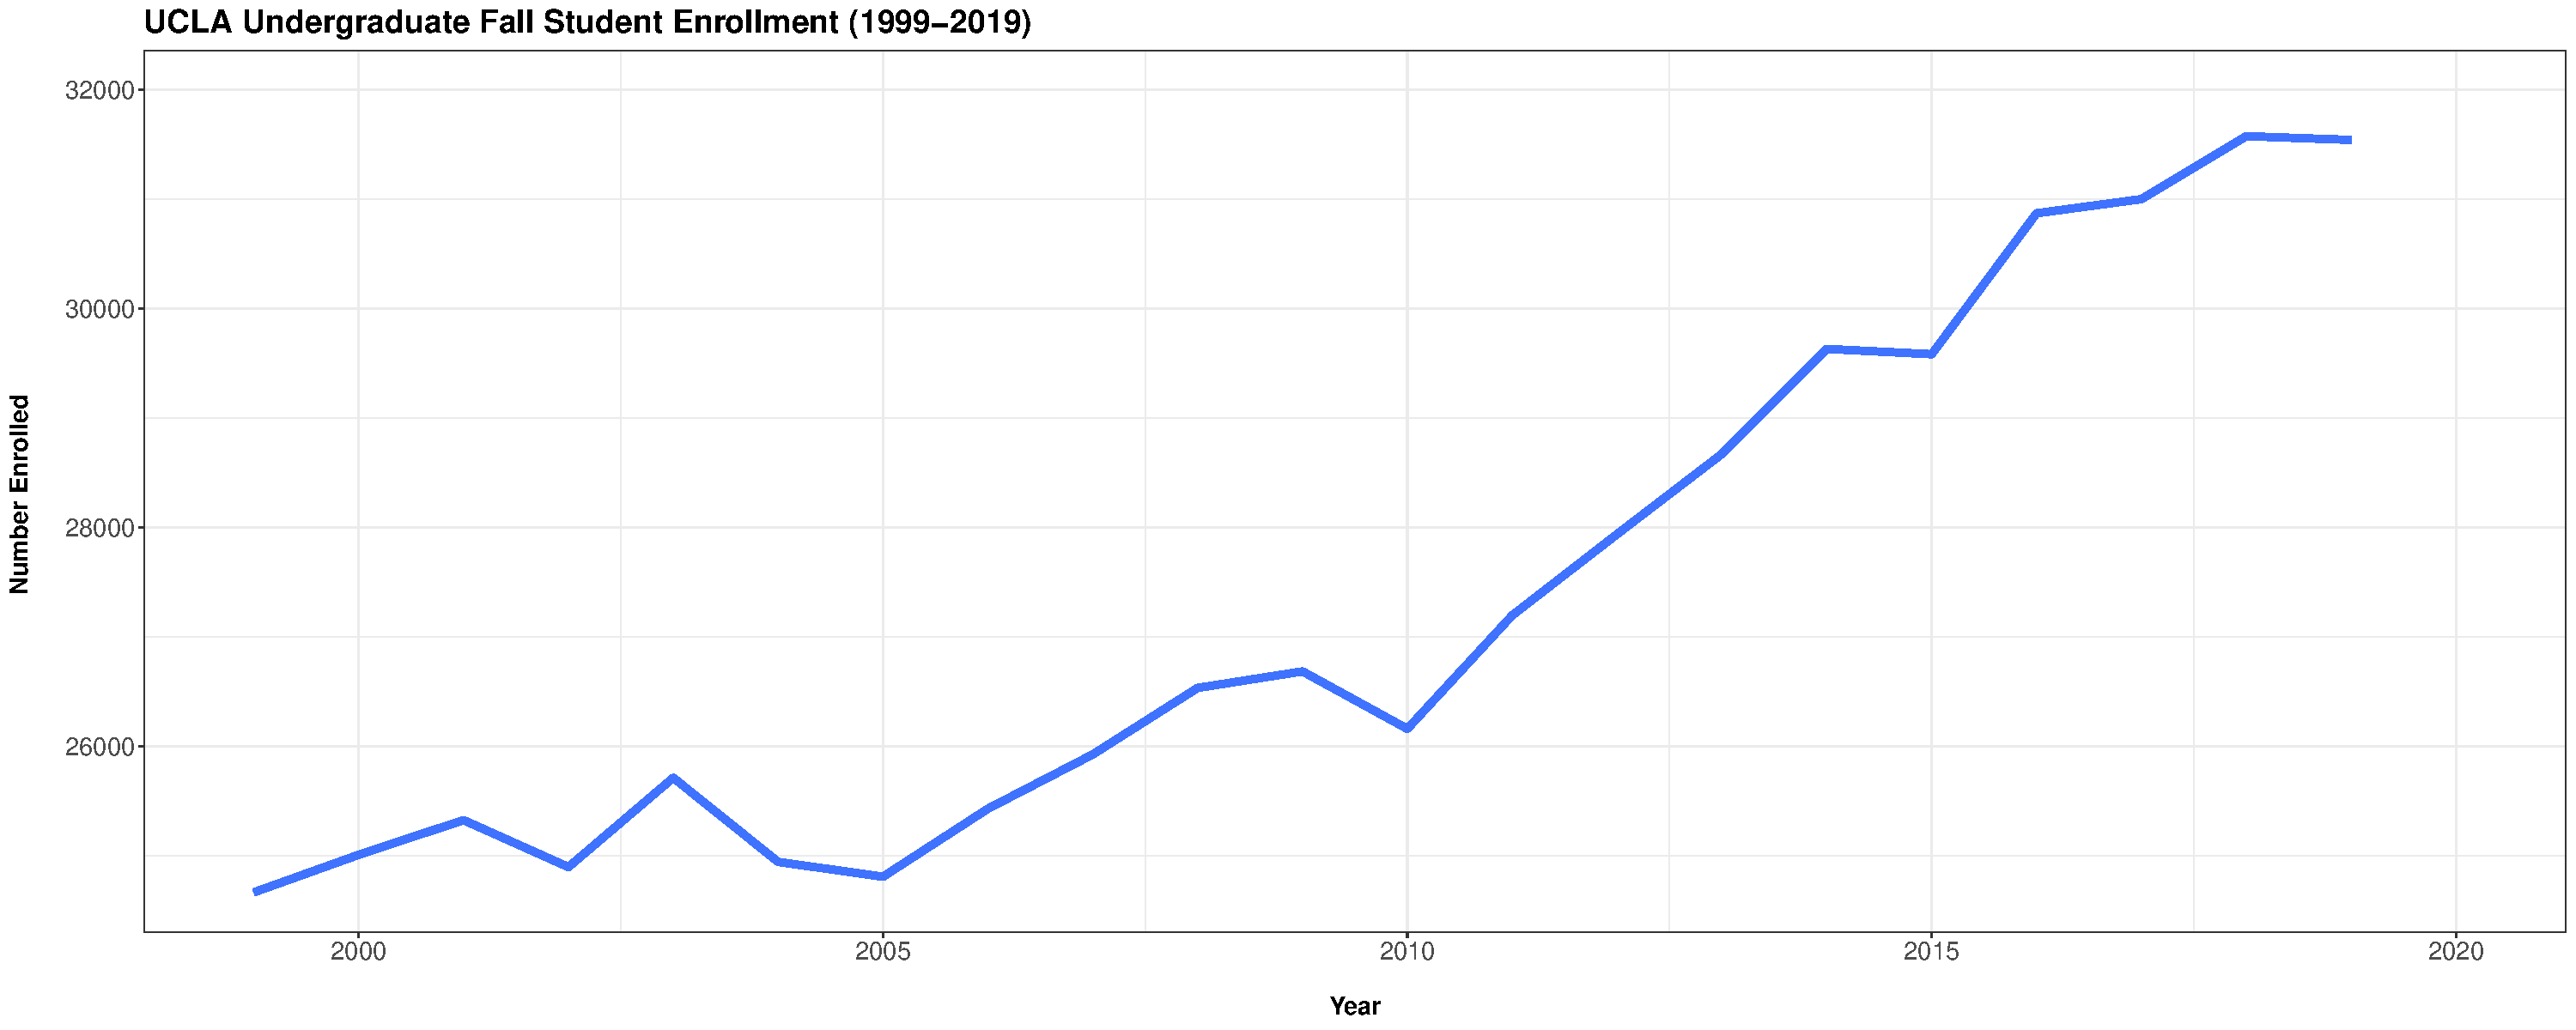
\includegraphics{index_files/figure-latex/fig1-1.pdf}

From the line plot alone, we can gather that enrollment numbers have
been trending upward year over year for the last 20 years. However, to
answer our original question: ``will we be seeing a notable decrease in
new student enrollments from 2019-2020?'' a t test with a confidence
level of 95\% is conducted below. Here, we are surmising that enrollment
numbers will be greater than or equal to 30,000. Alternatively, we are
postulating that the numbers will fall below 30,000. Let us now see the
results by plugging in the statistics we have calculated manually
earlier:

\begin{Shaded}
\begin{Highlighting}[]
\NormalTok{xbar =}\StringTok{ }\FloatTok{27340.48}
\NormalTok{mu0 =}\StringTok{ }\FloatTok{30000.00}
\NormalTok{sigma =}\StringTok{ }\FloatTok{2443.37}
\NormalTok{n =}\StringTok{ }\DecValTok{21}
\NormalTok{z =}\StringTok{ }\NormalTok{(xbar}\OperatorTok{-}\NormalTok{mu0)}\OperatorTok{/}\NormalTok{(sigma}\OperatorTok{/}\KeywordTok{sqrt}\NormalTok{(n))}
\NormalTok{z}
\end{Highlighting}
\end{Shaded}

\begin{verbatim}
## [1] -4.987968
\end{verbatim}

The z-value of -4.988 still holds true from our prior manual test, and
when calculated against alpha, we retrieve the critical value as follows

\begin{Shaded}
\begin{Highlighting}[]
\NormalTok{alpha =}\StringTok{ }\FloatTok{0.05}
\NormalTok{z.alpha =}\StringTok{ }\KeywordTok{qnorm}\NormalTok{(}\DecValTok{1}\OperatorTok{-}\NormalTok{alpha)}
\CommentTok{# The critical value (-z.alpha)is shown below}
\OperatorTok{-}\NormalTok{z.alpha}
\end{Highlighting}
\end{Shaded}

\begin{verbatim}
## [1] -1.644854
\end{verbatim}

The test statistic -4.988 is lower than the critical value of -1.645.
Therefore, at a 0.05 significance level, we must reject our initial
claim that student enrollment will reach or exceed 30,000 in the fall of
2020.

\begin{Shaded}
\begin{Highlighting}[]
\CommentTok{# t test of x against a null hypothesis}

\KeywordTok{t.test}\NormalTok{(enrollment}\OperatorTok{$}\NormalTok{Enrolled, }\DataTypeTok{mu =} \DecValTok{30000}\NormalTok{, }\DataTypeTok{conf.level =} \FloatTok{0.95}\NormalTok{)}
\end{Highlighting}
\end{Shaded}

\begin{verbatim}
## 
##  One Sample t-test
## 
## data:  enrollment$Enrolled
## t = -4.988, df = 20, p-value = 7.066e-05
## alternative hypothesis: true mean is not equal to 30000
## 95 percent confidence interval:
##  26228.27 28452.68
## sample estimates:
## mean of x 
##  27340.48
\end{verbatim}

As evident from the t-test above, the p-value of 3.553e-05 is
statistically significant, and falls substantially below the alpha level
of 0.05. As such, we must also reject the idea or notion that Fall
Student Enrollment in 2020 will equal or surpass that of 30,000 students
(the null hypothesis).

\end{document}
